% !TEX root =  master.tex
\chapter{Data}\label{chapter:data}

\section{NIH Data}\label{data:nih}
\sectionauthor{Written by Tobias Richstein}

The first of the datasets that we used to train our models comes from the \acf{NIH}, a division of the U.S. Department of Health, and is a collection of over 100 thousand chest X-ray images by over 30 thousand patients presented by \citeauthor{wang_chestx-ray8_2017} in \autocite{wang_chestx-ray8_2017}. This dataset was published in 2017 and is therefore not concerned with COVID-19 patients at all. Rather it consists of images depicting 14 different illnesses and images of healthy patients. The authors claim that there is a large amount of data in the form of patient X-rays and corresponding findings available in hospital's archiving systems but that these have not been properly consolidated and catalogued across multiple hospitals and states before. The authors also claim that the findings are mostly embedded in sentences making them not easily machine-readable.

To overcome these issues, the authors collected the images from different hospitals and used natural language processing to extract the medical findings from the written reports associated with the images. In the initial dataset this included eight different illnesses: Atelectasis, Cardiomegaly, Effusion, Infiltration, Mass, Nodule, Pneumonia and Pneumothorax as well as images with no finding at all. Later, the dataset was updated to the 15 class form (14 illnesses and no findings) that we use for our project to also include Consolidation, Edema, Emphysema, Fibrosis, Pleural Thickening and Hernia as findings. The class distribution can be seen in figure \vref{fig:nih_classes} where it is clear that the classes are very disproportionally represented. There is a total of $141,537$ diagnoses, meaning each image has an average of roughly $1.26$ labels associated. This number is skewed however since if anything is found then the average goes up to $1.56$ since no finding always means that only this one label is attached to a record.

\begin{figure*}
	\centering
	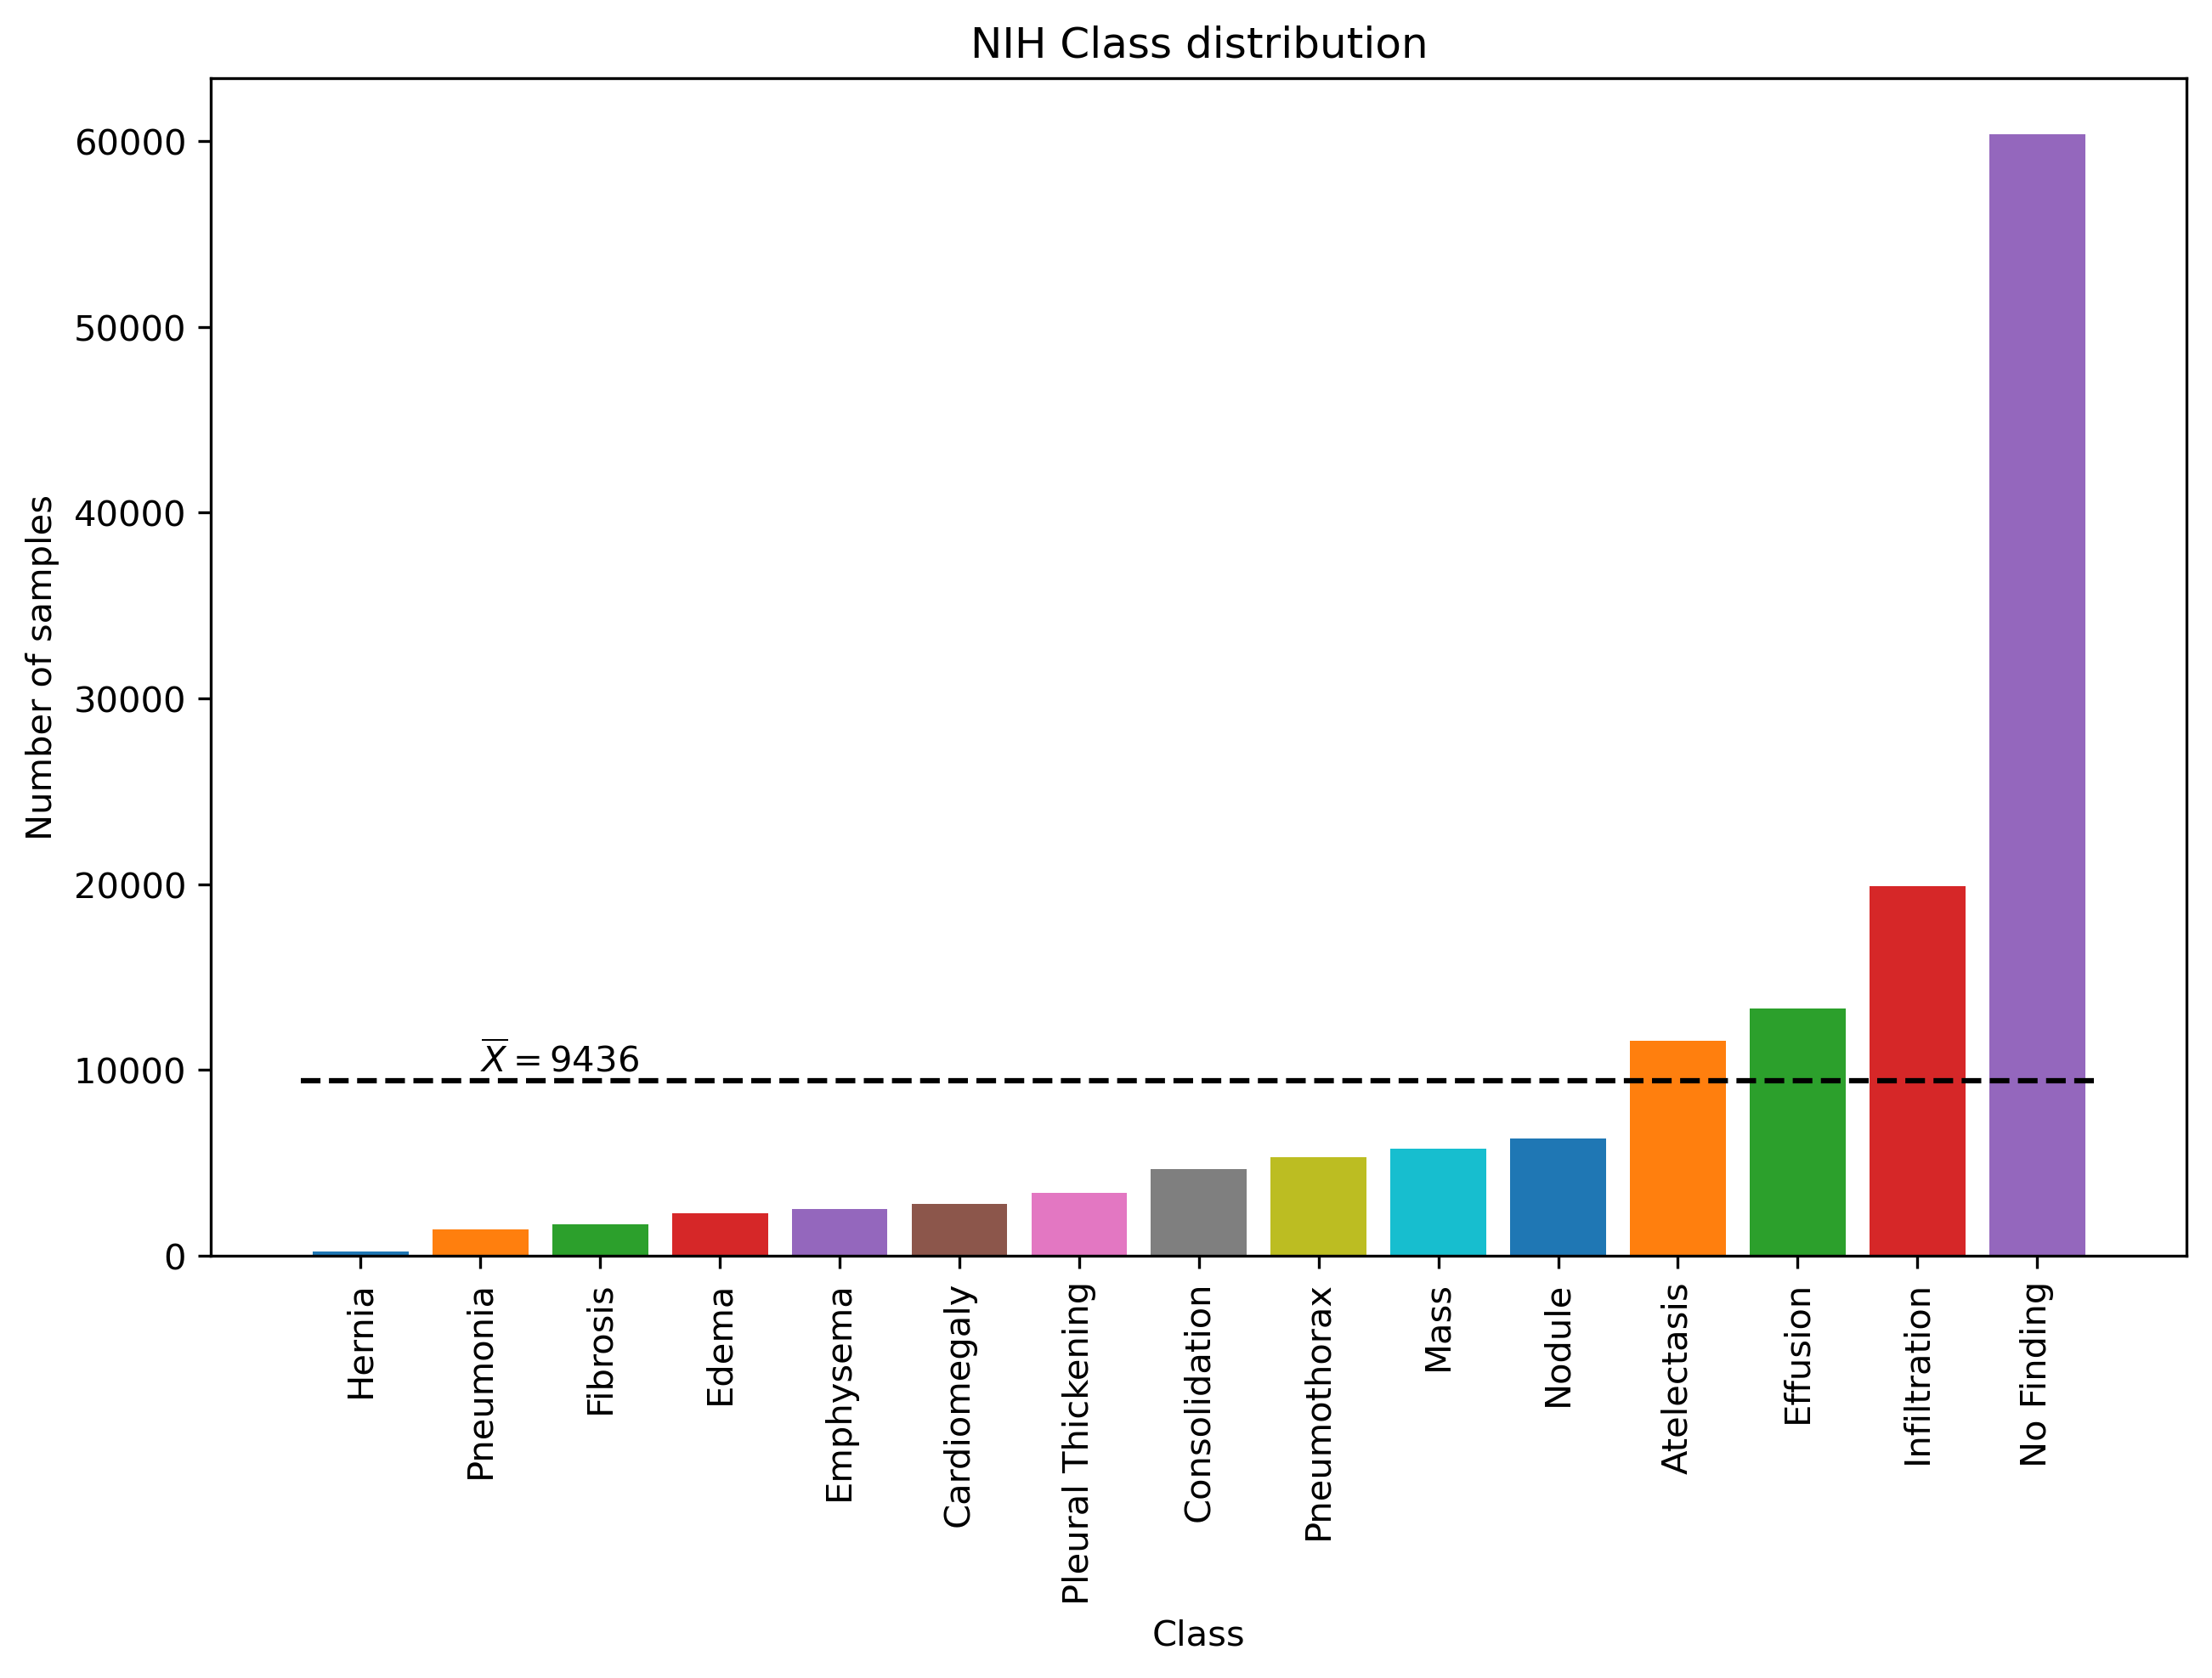
\includegraphics[width=.8\linewidth]{img/nih_class_distribution.png}
	\caption{Class distribution in the NIH dataset}
	\label{fig:nih_classes}
\end{figure*}

The images in the dataset are given in the PNG format and are all sized $1024 \times 1024$ and with RGB color channels. The dataset does have roughly six thousand entries for bounding boxes for some of the images but those are not really of use to us since there are so few and also because the value of this dataset lies somewhere else for us: The training of our backbone network for one of the object detection networks (more on that in section \vref{chapter:rcnn}). We can use this dataset to train the backbone on images that are roughly within the problem domain that we actually want to tackle so that the feature vectors that it produces are valuable to the actual object detection network. 

\section{RSNA Data}\label{data:rsna}
\sectionauthor{Written by Julian Seibel}

Similar to the pretraining of the Faster \ac{R-CNN} backbone on the above described NIH dataset, we use the RSNA dataset \autocite{RSNAKaeggle} originally published as part of a two-stage Kaggle challenge in 2018. The dataset contains $30,227$ samples from $26,684$ different patients in form of $1024 \times 1024$ DICOM images. Despite the data was anonymized, for every patient there are meta-information available including sex, age and radiographic view. The images were labeled by radiologists from \ac{RSNA} and the Society of Thoracic Radiology. There are three mutual exclusive  labels possible (lung opacity, normal, no lung opacity/ not normal) whereas lung opacity describes a indicates evidence for pneumonia including also bounding box information for regions of interest in the format $(x_{min}, y_{min}, width, height)$. A positive image can contain multiple bounding boxes. Figure \ref{fig:rsna_classes} shows the class distribution for the \ac{RSNA} datasets. In total there are $9,555$ sample images that are labeled as positive and therefore come along with labeled regions in form of bounding boxes.

The objective of this challenge was to train a model that is capable of correct classification including also bounding box predictions for each positive case and a confidence score, indicating the model confidence for a single bounding box prediction. The final submissions were evaluated using \ac{IoU} based metrics to measure the overlap of predicted and ground truth boxes. Figure \ref{fig:rsna_sample} shows an image from the \ac{RSNA} dataset including ground truth boxes (green), possible predictions (reds-dashed) and corresponding \ac{IoU} values.

Since this challenge has a lot in common with the challenge we want to contribute to in this work and the image appearance is the exact same, namely DICOM images of chest X-rays, we decided to include this dataset as additional source for pretraining our models. In contrast to the \ac{NIH} dataset, the \ac{RSNA} data is rather small, but brings one major advantage with labels including ground truth bounding boxes for positive pneumonia cases which makes the data suitable for pretraining object detection models. With this, we also think there are semantic similarities in predicting pneumonia and COVID-19 regions, that we hope will positively affect our final model performance for ultimately detecting COVID-19 evidence. In detail, we used the positive cases for training our detection models to \enquote{introduce} the weights into the domain of medical X-ray chest images. For the meta-data of the patients however, we did not find any suitable purpose which is why we ignored this information in the further course of this work.

\begin{figure*}
	\begin{minipage}[b]{.65\linewidth} % [b] => Ausrichtung an \caption
		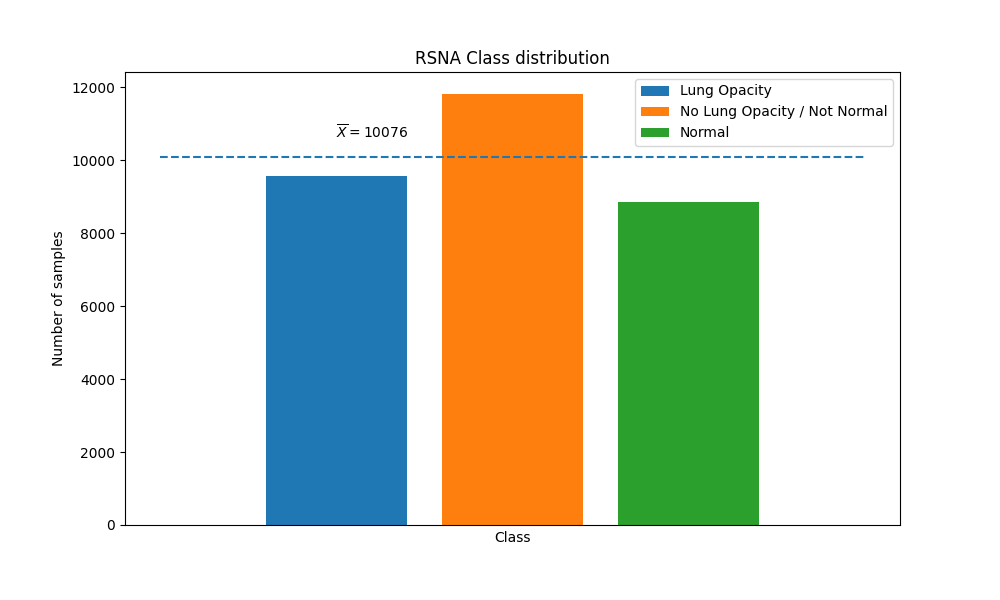
\includegraphics[width=\linewidth]{img/rsna_class_distribution.png}
		\caption{Class distribution in the RSNA dataset}
		\label{fig:rsna_classes}
	\end{minipage}
	\begin{minipage}[b]{.35\linewidth} % [b] => Ausrichtung an \caption
		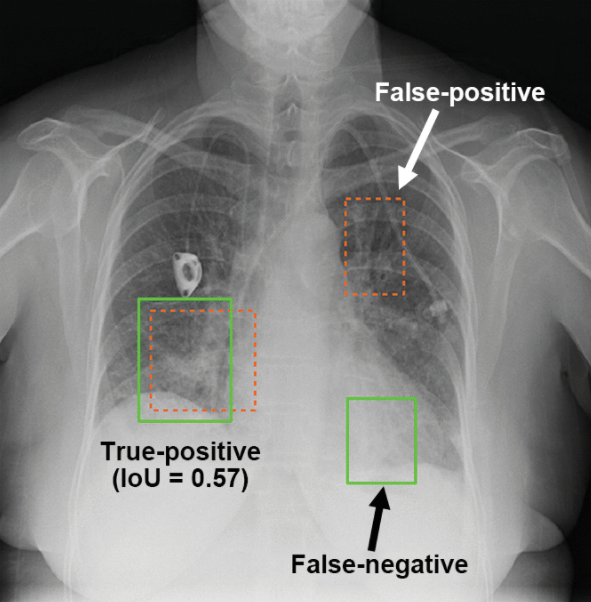
\includegraphics[width=\linewidth]{img/rsna_sample.png}
		\caption{Extracted from \autocite{rsnaSurvey}}
		\label{fig:rsna_sample}
	\end{minipage} 
\end{figure*}

\section{SIIM COVID-19 Data}\label{data:siim}
\sectionauthor{Written by Torben Krieger}

The last dataset we use is provided by the SIIM Kaggle Challenge itself \autocite{SIIMKaggle}. It contains \ac{CXR} images of COVID-19 positive and negative patients. The dataset itself is a reassembly of at least two previously published datasets. Namely the \textit{BIMCV-COVID19 Data} initially published by \citeauthor{vaya2020bimcv} in June 2020 \autocite{vaya2020bimcv} and the \textit{RSNA MIDRC-RICORD Data} published by \citeauthor{tsai2021rsna} in January 2021 \autocite{tsai2021rsna}. Only the X-ray images were taken from both datasets the annotation of the data was recreated for the assembled dataset. Both datasets were refreshed and supplemented multiple times. The description of the Kaggle Challenge not specifies which versions were used for the assembly.

The initial version of the \textit{BIMCV-COVID19} dataset contains 1,380 CR images and 885 DX images \autocite{vaya2020bimcv}. Generally we do not distinguish between the two classical X-ray modalities CR and DX, thus the dataset contains 2265 CXR images. The images were taken from 1,311 unique COVID-19 positive patients in hospitals within the region of Valencia, Spain. All images are provided in the DICOM format including metadata, although anonymized for privacy reasons. Nevertheless patients age and sex was retained. The original dataset includes additional data, e.g. the results of one or multiple COVID-19 tests (at least one positive) and a corresponding radiological report.

The \textit{MIDRC-RICORD} dataset contains 1000 CXR images of 361 unique COVID-19 positive patients \autocite{tsai2021rsna}. Where positive means that at least one \ac{RT-PCR} test was positive for the corresponding patient. The data was collected from four different hospitals in Istanbul, San Francisco, Toronto and São Paulo and is provided in DICOM format including metadata, again anonymized. Also here patient sex and age was retained, the authors specify that 148 out of the total amount of patients is female (41\%).

As stated above the Kaggle dataset is a combination of the datasets described before. As both datasets contain CXR images for positive tested patients only, there has to be at least one additional data source. Unfortunately the description of the challenge does not provide any details about this or the exact collocation of the assembled dataset. The new dataset was annotated by professional radiologists. Per image opacities were marked with bounding boxed if found. On study level a classification into the categories, as described in section \ref{sec:kaggle}, were done by the radiologists. The classification follows the schema described by \citeauthor{litmanovich2020review} where each class is mutual exclusive \autocite{litmanovich2020review}. It is crucial to emphasize that radiologists had access to the COVID-19 status while creating the annotations \autocite{SIIMKaggleAnnotation}.

The dataset consists out of a train and test set, however the test labels are not published. A test is only possible by submitting a solution as notebook. As we decided that we will not hand in our results, and use supervised methods only, we are limited to the train set for this report. The train set contains 6,334 images, all images are provided in the DICOM format. Metadata is available but anonymized. Out of the patient data only the patient sex was retained. All DICOM image files of the train set have a uncompressed size on disk of 108.2 GB after the download. The images belong to 6054 studies. The count of unique patients could not be extracted from the anonymized metadata and is not specified. The resolution of the images reaches from 846 to 4,891 pixel rows and 1,228 to 4,891 pixel columns. All images are single channel greyscale images. The DICOM standard defines different representations for image pixel data, so called \textit{Photometric Interpretations} \autocite{dicom2018}. Within the dataset we could find 4,633 images with the \texttt{MONOCHROME2} representation, which means that the minimum pixel value should be interpreted as black. Contrary 1,701 images are encoded with \texttt{MONOCHROME1} representation, minimum pixel value means white color here. In DICOM modalities could store a custom amount of bits per pixel value, which relates to the bit depth of the greyscale channel in our case. Figure \ref{fig:dicom-bits-stored} shows an overview of the different bit depths found for images within the dataset. For training it is required to convert the pixel data of all files to a single representation and bit depth. Specifically by reducing the bit depth we lose some information which is might relevant for good predictions. Most of the included DICOM files contain uncompressed pixel data, only 440 files hold the pixel data compressed using the JPEG Lossless format. As expected the DICOM metadata field specifying the examined body part indicates \enquote{CHEST} most often, although encoded in different languages (e.g. \enquote{THORAX}, \enquote{PECHO}). However some unexpected values are included, e.g. 57 files claim \enquote{SKULL} as examined body part. We checked some of these files manually, it seems that this is rather a misconfiguration of the modality. All images checked have shown the chest of the screened patients. For the complete train dataset 2,770 images were taken of female patients, 3,564 of male patients.

// todo figure bit width

Most of the 6,054 studies were classified as \textit{Typical Appearance} (2,855 occurrences). In contrast to this the class \textit{Atypical Appearance} has only 474 occurrences, which is roughly a sixth of most frequent class. Thus the dataset is imbalanced with respect to a domination of potential COVID-19 positive samples. Figure \ref{fig:study-class-distribution} shows the complete class distribution within the train set. In addition figure \ref{fig:class-samples} shows some sample images per class. Per description of the challenge for the classes \textit{Typical} and \textit{Indeterminate} bounding boxes marking opacities should be present always \autocite{SIIMKaggleAnnotation}. Contrary to that for the negative class no bounding boxes were created. For \textit{Atypical Appearances} sometimes a bounding box is included. In total we found 2,040 images without any bounding box / opacity. Figure \ref{fig:boxes-per-images} shows an overview on the count of boxes per image. Most were annotated with two opacities. The figure \ref{fig:boxes-size} prints the number of boxes over the box size, thus giving an impression on the box sizes within the images. Related to this the description says that the radiologists opted for a single larger bounding boxes when multiple adjacent opacities were found, rather than creating multiple smaller boxes \autocite{SIIMKaggleAnnotation}. Bounding boxes for the image level and classes per study are provided in two separate CSV files.

// todo study class distribution figure
// todo boxes per image (+counts)
// todo box sizes

Already by the construction of the dataset itself we could foresee potential issues with regards to the real generalization capability of trained models. Most importantly the dataset is constructed out of several sources, where specific sources provided positive or negative samples only. Thus it could be that a potential solution learns shortcuts introduced by the processes or equipment used by a specific image source. An example could be burned in image markers at a specific position of the X-ray. We were able to find some re-occurring burned-in markers at the same position for a couple of images within the dataset. The next problem are the facts we do not know about the dataset, e.g. the age distribution or the position of the patient while retrieving the X-ray scan. For example one could imagine that images retrieved in a lying position correspond to more severe and potential positive cases. All the critical points described before were mentioned within a paper by \citeauthor{degrave2021ai} \autocite{degrave2021ai} this paper explicitly investigated the \textit{BIMCV-COVID19} dataset and found the aforementioned shortcomings therein. As the Kaggle dataset is a reassembly of this dataset we have to expect that these issues are also present within it. Additionally we only have very limited information about the construction process of the dataset. Summing up a comprehensive conclusion about the generalization capability of our methods will not be possible by using this dataset.

\subsection*{Preprocessing of the dataset \& COCO}
Independent of the applied model or task we applied a first preprocessing to the dataset. In general we apply the following to each DICOM image file:
\begin{itemize}
	\item Applying VOI-LUT, if present within DICOM metadata. This is a necessary pixel value transformation for some modalities to transform pixel values retrieved by the X-ray detector to a specific representation for displaying the image \autocite{dicom2018}. Not all DICOM files come with a VOI-LUT attribute.
	\item Inverting pixel values for \texttt{MONOCHROME1} images. By doing so we make sure that all pixel values within the images comply to the \texttt{MONOCHROME2} representation, meaning the minimum value is interpreted as black.
	\item Rescale all greyscale pixel values to a value range of $[0,255]$ to represent them with a bit depth of 8 bit.
	\item Store each image as lossless compressed grayscale image using the \ac{PNG} file format.
\end{itemize}

By applying the above mentioned preprocessing steps we reduced the overall size of the dataset to 25 GB. We also dropped all DICOM metadata as we do not require these information for the training and evaluation process. Still it is worth to mention again that the rescale of all image pixel data to a bit depth of 8 bit implies a significant loss of image information. However as we require to use pre-trained models for this project this is definitely required.

For the object detection task on image level we need a specific format of annotation to make use of several pre-trained models. This format is specific to the Microsoft \ac{COCO} dataset initially described by \citeauthor{lin_microsoft_2015} in \citeyear{lin_microsoft_2015}. This dataset is one of the largest and commonly used dataset for object detection, segmentation and captioning. Due to that fact most pre-trained models for these tasks were trained using this dataset. To reuse these pre-trained models easily for other tasks the custom dataset has to comply to the label format used within the \ac{COCO} dataset.


\begin{minipage}{\linewidth}
	\begin{lstlisting}[language=json,firstnumber=1, caption={Basic COCO annotation format in \autocite{lin_microsoft_2015}}, captionpos=b, label={lst:coco-sample}]
{
  "images": [
    { "id": int, "width": int, "height": int, "file_name": str,"date_captured": datetime }, (..)
  ], 
  "annotations": [
    { "id": int, "image_id": int, "category_id": int, "area": float, "bbox": [x,y,width,height] }, (..)
  ],
  "categories": [
    { "id": int, "name": str }, (..)
  ]
}
	\end{lstlisting}
\end{minipage}

The label format is defined as JSON format, listing \ref{lst:coco-sample} shows the most important content nodes and attributes for our task.
The node \texttt{images} contains per image one entry, the \texttt{file\_name} attribute could be a relative path. The node \texttt{annotations} contains a single node per bounding box for any image.
We provide functionality to convert the image level CSV file provided by the Kaggle dataset into a single JSON file which conforms to the \ac{COCO} format.

